\documentclass[12pt,a4paper]{article}
\usepackage[utf8]{inputenc}
\usepackage[english]{babel}
\usepackage{amsmath}
\usepackage{amsfonts}
\usepackage{amssymb}
\usepackage{graphicx}
\usepackage{lmodern}
\usepackage[left=2cm,right=2cm,top=2cm,bottom=2cm]{geometry}
\usepackage{tikz}
\usepackage{todonotes}

\author{Chowdhury Amir Abdullah}


\begin{document}


\begin{tikzpicture}
\draw (0,0) -- (1,1); % a line
\end{tikzpicture}\\[6pt]



\begin{tikzpicture}
\draw[help lines] (0,0) grid (3,3);
\end{tikzpicture}\\[6pt]



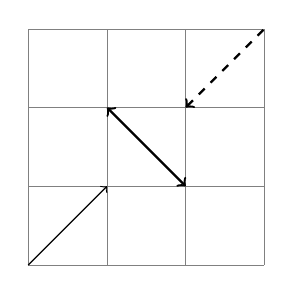
\begin{tikzpicture}
\draw[help lines] (0,0) grid (3,3);
\draw[->] (0,0) -- (1,1);
\draw[<->, thick] (2,1) -- (1,2);
\draw[<-, thick, dashed] (2,2)--(3,3);
\end{tikzpicture}\\[6pt]



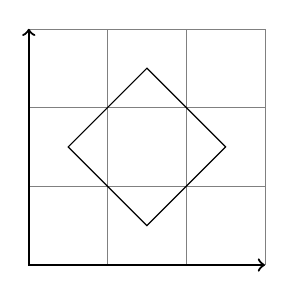
\begin{tikzpicture}
\draw[help lines] (0,0) grid (3,3);
% axes:
\draw[<->, thick] (0,3)--(0,0)--(3,0);
% diamond:
\draw (1.5,0.5) -- (2.5,1.5) --
(1.5,2.5) -- (0.5,1.5) --
cycle; % close the path
\end{tikzpicture}\\[6pt] 




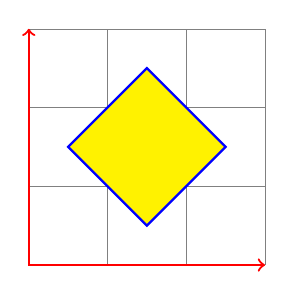
\begin{tikzpicture}
\draw[help lines] (0,0) grid (3,3);
% axes
\draw[<->, thick, red]
(0,3)--(0,0)--(3,0);
% diamond
\draw[thick, blue, fill=yellow]
(1.5,0.5) -- (2.5,1.5) --
(1.5,2.5) -- (0.5,1.5) --
cycle;
\end{tikzpicture}\\[6pt]




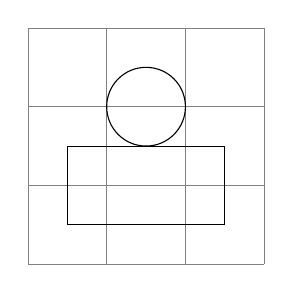
\begin{tikzpicture}
\draw[help lines] (0,0) grid (3,3);
\draw (1.5,2.0) circle (0.5);
\draw (0.5,0.5) rectangle (2.5,1.5);
\end{tikzpicture}\\[6pt]



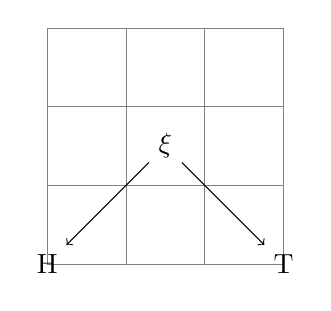
\begin{tikzpicture}
\draw[help lines] (0,0) grid (3,3);
\node (h) at (0,0) {H};
\node (x) at (1.5,1.5) {$\xi$};
\node (t) at (3,0) {T};
\draw[->] (x) -- (h);
\draw[->] (x) -- (t);
\end{tikzpicture}\\[6pt]



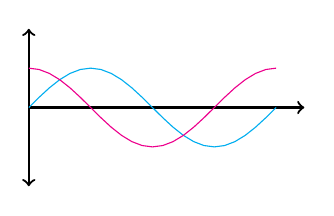
\begin{tikzpicture}[scale=0.5]
% y axis
\draw[<->, thick] (0,2) -- (0,-2);
% x axis
\draw[ ->, thick] (0,0) -- (7, 0);
% curves
\draw[cyan,domain=0:2*pi]
plot (\x, {sin(\x r)});
\draw[magenta,domain=0:2*pi]
plot (\x, {cos(\x r)});
\end{tikzpicture}\\[6pt]


\todo{add results}
\todo[color=blue!20]{fix method}

\newcommand{\alice}[1]{\todo[color=green!40]{#1}}
\newcommand{\bob}[1]{\todo[color=purple!40]{#1}}
\alice{add results}
\bob{fix method}

\end{document}